\newpage
\appendix

\chapter{The Exo-FMS GCM}\label{ap:exo-fms}


% 0 -- LEAD-IN PARAGRAPHS

%START ELEMENT

A General Circulation Model (GCM) simulates the fluid dynamics of an atmosphere or ocean, coupled to other models of physical processes such as radiative transfer or convection. GCMs are valuable tools for investigating the atmospheric dynamics of new types of exoplanet, as they can simulate a great variety of planetary atmospheres without prior knowledge. This appendix reviews the structure and functionality of the GCM ``Exo-FMS'' used to model planetary atmospheres in this thesis. Exo-FMS is hosted at \url{github.com/OxfordPlanetaryClimate}, and will be made public soon.


\section{Model Structure}

Exo-FMS has a simple structure with as few changes as possible to the original code release of the latest cubed-sphere version of the GFDL FMS\footnote{\url{gfdl.noaa.gov/cubed-sphere-quickstart}}. In this section, I will give an overview of the modelling structure ``FMS'', the dynamical core and physics modules, and the ``Exo-FMS'' interface between the dynamical core and physics modules.


\subsection{FMS}

Exo-FMS is built on the GFDL ``Flexible Modelling System'' (FMS)\footnote{\url{gfdl.noaa.gov/fms}}, which is a ``software framework for supporting the efficient development, construction, execution, and scientific interpretation of atmospheric, oceanic, and climate system models''. In the context of Exo-FMS, FMS is the framework of the model, which manages the compiling and running of the model, data input and output, parallelisation via MPI, and many utilities such as time-keeping or initialisation.


\subsection{Physics Interface}

Exo-FMS is based on a single interface between the dynamical core and the physics modules. The interface takes the state of the atmosphere at each timestep (its temperature, pressure, and so on) and passes it to each module in turn. These each return a tendency in some variable (a temperature tendency from the radiative transfer scheme, for example) which are then applied to the atmospheric state.

I produced this interface to simplify the addition of new physics modules to the model. The interface also makes it simple to swap the modules in and out, to model different types of planet. This is very valuable for simulating exoplanets that may have different processes at work in their atmospheres. Developing the new interface allowed more use of the object-oriented style of the recent release of the FMS, giving a more straightforward coupling between the dynamical core and physics modules.


\subsection{Physics Modules}

The default configuration of the unmodified cubed-sphere release of the FMS couples the dynamical core to a single physics module that applies a ``Held-Suarez'' forcing scheme \citep{held1994proposal}. Exo-FMS includes additional modules to simulate different physical processes, which can be swapped in and out using the interface discussed above.

The simplest configuration applies dry convective adjustment, a Rayleigh drag at the surface, and semi-grey radiative transfer \citep{pierrehumbert2010principles}. This configuration was used for the simulations in Chapters \ref{ch:eqm-zonal-flow} and \ref{ch:wave-mean-flow}. Chapter \ref{ch:linking-climate-55cnce} used the same configuration of modules in the previous version of Exo-FMS on latitude-longitude grid. The simulations in Chapter \ref{ch:clouds-lava-planets} use the new cubed-sphere version of Exo-FMS with the more realistic radiative transfer model \textit{Socrates} \citep{edwards1996socrates}. The  cloud formation and transport model DIHRT has also been coupled to Exo-FMS \citep{lee2016dynamic}. The next steps in the model development will be to add more detailed convective adjustment schemes or to couple it to a chemical model.


\subsection{Utilities}

I also produced Python utilities to run the model and process its output. The Python interface to run the model provides a single script to set its input parameters. The interface then produces the model runscript, several Fortran namelists to set the parameters of the test, and sets the model diagnostics that will be saved. After the test finishes, the interface then uses the ``cubedsphere'' Python package\footnote{\url{github.com/JiaweiZhuang/cubedsphere}} to re-grid the diagnostic fields from a cubed-sphere grid to a latitude-longitude grid for analysis.


\section{Finite-Volume Dynamical Core}

The dynamical core of the model solves the primitive equations describing the fluid dynamics of the atmosphere \citep{lin2004fv, vallis2006book}. A finite-volume core (as opposed to a finite-difference core, or a spectral core) uses a grid of points, each with a surrounding volume that exchanges fluxes with the adjacent volumes.

\subsection{Latitude-Longitude}

The simulations in Chapter \ref{ch:linking-climate-55cnce} used a version of Exo-FMS inherited from \citet{pierrehumbert2016dynamics}. The dynamical core of this version was on a latitude-longitude grid, shown in Figure \ref{fig:gcm-grids-ll}. It became clear that the poles of this grid were a source of instability for the high temperature and high winds produced in simulations of 55 Cancri e. The instability was likely due to a failure of the CFL condition at the poles, which requires that

\begin{equation}
  C=\frac{u \Delta t}{\Delta x} \leq C_{\max },
\end{equation}

where $u$ is the local velocity, $\Delta t$ is the model timestep, $\Delta x$ is the local grid scale, $C$ is the Courant number, which must be below a critical value $C_{max}$ \citep{courant1928partiellen}. On a latitude-longitude grid, the grid scale $\Delta x$ becomes very small at the poles, requiring a very small timestep $\Delta t$ to satisfy this condition. I therefore updated the model to use a newer dynamical core on a cubed-sphere grid, which does not have such a small grid scale at its poles.


\begin{figure}
  \centering
  \begin{subfigure}[t]{0.37\textwidth}
    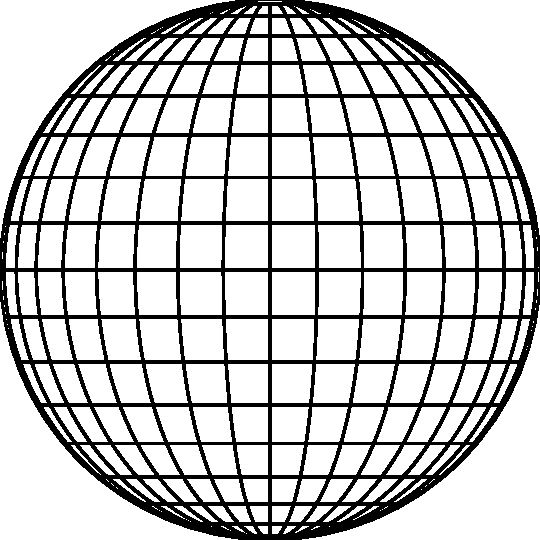
\includegraphics[width=1.0\textwidth]{figures/appendices/lat-lon-grid.pdf}
    \caption{Latitude-longitude grid.}
    \label{fig:gcm-grids-ll}
  \end{subfigure}
  %
  \quad\quad\quad
  \begin{subfigure}[t]{0.37\textwidth}
    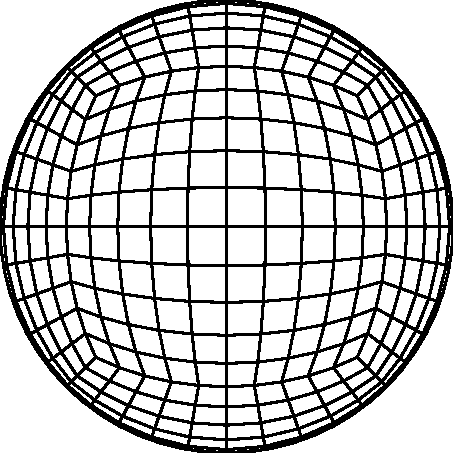
\includegraphics[width=1.0\textwidth]{figures/appendices/cubed-sphere-grid.pdf}
    \caption{Cubed-sphere grid.}
    \label{fig:gcm-grids-cs}
  \end{subfigure}
  \caption{The old latitude-longitude grid and the new cubed-sphere grid used in Exo-FMS. The new grid avoids the small grid scale at the poles of the old grid, which was a source of instability.}
  \label{fig:gcm-grids}
\end{figure}

\subsection{Cubed-Sphere}

Figure \ref{fig:gcm-grids-cs} shows a cubed-sphere grid like the grid used in the updated version of Exo-FMS \citep{putman2007cubed}. A cubed-sphere grid is a regular grid on the six faces of a cube that is projected onto the surface of a sphere. This creates six ``poles'' on the grid from the vertices of the cube, as well as small variations in the grid cell sizes. These can produce instabilites at the poles, or artifacts in the pattern of the grid \citep{putman2007cubed}, but these were never a serious issue in the simulations in this thesis. The updated version of Exo-FMS was found to avoid the instabilities and crashing caused by high winds at the poles of the latitude-longitude grid, and to run more stably which allowed for longer timesteps.




% %SECTION 4 -- PLANETS
% \section{Example Planets}
%
% %SUBSECTION -- TEMPERATE TERRESTRIAL PLANETS
% \subsection{Temperate Terrestrial Planets}
%
%
% %SUBSECTION -- LAVA PLANETS
% \subsection{Lava Planets}
%
%
% %SUBSECTION -- GAS PLANETS
% \subsection{Gas Planets}







%%%%%%%%%%%%

% \chapter{GFDL-SDC}\label{ap:gfdl-sdc}
%
% The non-linear shallow-water simulations in Chapter X were run using the Geophysical Fluid Dynamics Laboratory Spectral Dynamical Core (GFDL-SDC).
%
% \section{Model Details}
%
% The GFDL-SDC uses a spectral solver.
%
% \section{Simulation Details}
%
% I used a shallow-water variant of the GFDL-SDC, with a single layer following the shallow-water equations:
%
% The tests in Figure X were forced by a relaxation to the height field X, the same as the linear theory in Chapter X.
%
% The tests in Figure X also had a zonal acceleration applied with the form X, the same as the tests of the linear theory in Chapter X.

% \section{Thesis Experiment Run Parameters}
%
% All of the experiments run in the cubed-sphere version of Exo-FMS are available online at X, in the format X described above.
%
% The experiments in Chapter X and Figure X in Chapter X were run in the older latitude-longitude version of Exo-FMS. Experiments in the new Exo-FMS X format are available as examples in the same location, giving a setup with the same physics and planetary parameters.


%%%%%%%%%%%


\chapter{Pseudo-Spectral Methods for the Shallow-Water Equations}\label{ap:ps-methods}

This appendix describes the pseudo-spectral methods used to solve the linearised shallow-water equations in Chapters \ref{ch:eqm-zonal-flow} and \ref{ch:wave-mean-flow}. I will give a general description of a pseudo-spectral collocation method, then show the methods used to solve the shallow-water equations on the beta-plane and on a sphere.

\section{Pseudo-Spectral Collocation for a Single Equation}

A pseudo-spectral collocation method expands the solution to a partial differential equation or system of equations as a series of ``basis functions'' and then imposes the condition that the equation is satisfied at a number of ``collocation points'' \citep{boyd2000spectral}. The resulting matrix equation provides the coefficients of the series, giving the solution to the initial equation.

For a linear ordinary differential equation:

\begin{equation}\label{eqn:ps-original-eqn}
  L u = q
\end{equation}

where $L$ is a differential operator acting on the variable $u$, and $q$ is the forcing or eigenvalue term, the solution is written as a sum of a series of basis functions:

\begin{equation}\label{eqn:pseudospectral_sum}
  u(x) = \sum a_{n} \psi_{n}(x).
\end{equation}

This is solved by imposing the condition that the differential equation is satisfied at $N$ ``collocation points'', the positions of which depend on the set of basis functions. The condition is equivalent to specifying that the ``residual'' -- the difference between the exact solution and the pseudo-spectral series solution -- is zero at these points. This provides $N$ equations to solve for the $N$ unknowns $a_{n}$, which gives the matrix equation:

\begin{equation}\label{eqn:ps_matrix}
 \textbf{H} \textbf{a} = \textbf{f},
\end{equation}

where the matrix elements $H_{ij}$ are the operator $L$ applied to the modes $\phi_{j}$ at the collocation points $x_{i}$, and the vector elements $f_{i}$ are the right-hand-side forcing terms $q$ evaluated at the collocation points $x_{i}$:

\begin{equation}\label{eqn:ps_H}
  H_{ij} = L \phi_{j}(x_{i}),
\end{equation}

\begin{equation}
  f_{i} = q(x_{i}).
\end{equation}

Solving Equation \ref{eqn:ps_matrix} with a numerical method such as LU decomposition gives the coefficients $a_{n}$ of the solution $u(x)$.



\section{Beta-Plane Shallow Water Equations}\label{sec:app-systems}

% The shallow-water equations on the beta-plane can be solved directly without reduction to a tidal equation. This allows the used of parabolic cylinder functions to represent each variable, which correspond to the exact solutions with zero background flow. So, while the above solution of the tidal equation with Chebyshev functions applies more generally, this specific solution with parabolinc cylinder functions can be exactly correct and can provide more insight into the effect of background flow on the modes of the system.

% The pseudo-spectral method can also be applied to systems of linear ordinary differential equations.

The method above can be applied to a system of equations rather than a single equation. Equation \ref{eqn:ps-original-eqn} is modified so that $L$ is a matrix and $u$ and $q$ are vectors. In the case of a system of forced, time-independent equations:

\begin{equation}\label{eqn:ps-multi-eqns}
  \textbf{L} \textbf{u} = \textbf{q},
\end{equation}

the condition that the differential equation is satisfied at the collocation points gives the equivalent matrix equation to Equation \ref{eqn:ps_matrix}:

\begin{equation}
  \textbf{H} \textbf{a} = \textbf{f}.
\end{equation}

$\textbf{H}$ is an $M \times N$ square matrix with elements:

\begin{equation}
  H^{kl}_{ij} = L^{kl}\phi_{j}(x_{i}),
\end{equation}

i.e. the operator $L^{kl}$ acting on the $l$th variable in the $k$th equation, applied to the $j$th basis function and evaluated at the $i$th collocation point. $\textbf{f}$ is a vector made up of $N$ subvectors $f_{i}$, which are the forcing terms in each equation evaluated at each collocation point.

\begin{equation}
    \textbf{H} =
  \begin{pmatrix}
    \begin{pmatrix}
H_{ij} & \dots \\
\vdots & \ddots
    \end{pmatrix}^{kl} & \dots \\
  \vdots & \ddots
  \end{pmatrix}
  \begin{pmatrix}
    \begin{pmatrix}
    \alpha_{i} \\
    \vdots
    \end{pmatrix} \\
  \vdots
  \end{pmatrix}
  =
  \begin{pmatrix}
    \begin{pmatrix}
    f_{i} \\
    \vdots
    \end{pmatrix} \\
  \vdots
  \end{pmatrix}.
\end{equation}

$\textbf{H}$ is the same as the matrix in Equation \ref{eqn:ps_H} with the elements $H_{ij}$ replaced by submatrices $H^{kl}_{ij}$. Solving this system returns the coefficients of the basis functions, and the solutions are:

\begin{equation}\label{eqn:ps-coeff-solutions}
 u(y) = \sum_{n=0}^{N} a_{n} \phi_{n}
; \quad
 v(y) = \sum_{n=0}^{N} b_{n} \phi_{n}
; \quad
 h(y) = \sum_{n=0}^{N} c_{n} \phi_{n}.
\end{equation}


This gives a linear matrix equation with one solution corresponding to the coefficient vectors $a_{n}$, $b_{n}$, $c_{n}$ of the forced solution.

For the forced linear shallow-water equations, the matrix equation \ref{eqn:ps-multi-eqns} corresponds to Equation \ref{eqn:sw-eqns-forced} in Chapter \ref{ch:eqm-zonal-flow} \citep{matsuno1966quasi}. These can be solved using the parabolic cylinder functions plotted in Figure \ref{fig:hermite-functions}. These functions are appropriate as they obey the boundary conditions of the beta-plane linear shallow-water equations, and the lowest order functions are exact solutions of the shallow-water equations.

Without forcing, the shallow-water equations define a free eigensystem where the eigenvalue is the frequency $\omega$.

\begin{equation}\label{eqn:ps-sw-eigenvalue}
  \textbf{L} \textbf{u} = \omega \textbf{P} \textbf{u}.
\end{equation}

The pseudo-spectral equation is then:

\begin{equation}
  \textbf{H} \textbf{a} = \omega \textbf{R} \textbf{a},
\end{equation}

 where $\textbf{R}$ is an $M \times N$ square matrix with elements:

\begin{equation}
  R^{kl}_{ij} = P^{kl}\phi_{j}(x_{i}),
\end{equation}

i.e. the eigenvalue operator $P^{kl}$ acting on the $l$th variable in the $k$th equation, applied to the $j$th basis function and evaluated at the $i$th collocation point:

\begin{equation}
    \textbf{H} =
  \begin{pmatrix}
    \begin{pmatrix}
H_{ij} & \dots \\
\vdots & \ddots
    \end{pmatrix}^{kl} & \dots \\
  \vdots & \ddots
  \end{pmatrix}
  \begin{pmatrix}
    \begin{pmatrix}
    \alpha_{i} \\
    \vdots
    \end{pmatrix} \\
  \vdots
  \end{pmatrix}
  =
  \omega
  \begin{pmatrix}
    \begin{pmatrix}
R_{ij} & \dots \\
\vdots & \ddots
    \end{pmatrix}^{kl} & \dots \\
  \vdots & \ddots
  \end{pmatrix}
  \begin{pmatrix}
    \begin{pmatrix}
    \alpha_{i} \\
    \vdots
    \end{pmatrix} \\
  \vdots
  \end{pmatrix}.
\end{equation}

This means that Equation \ref{eqn:ps-sw-eigenvalue} is a solvable eigenvalue matrix equation, with $N$ eigenvalues and eigenvectors, corresponding to the frequencies and coefficient vectors $a_{n}$, $b_{n}$, $c_{n}$ for each free mode. It can be solved with a similar numerical solution to the linear matrix equation in the forced problem. Not all $N$ modes must be physically realistic, so the spurious modes are identified by inspecting the eigenvalues for different values of $N$.


\begin{figure}
  \centering
  \begin{subfigure}[b]{0.48\textwidth}
    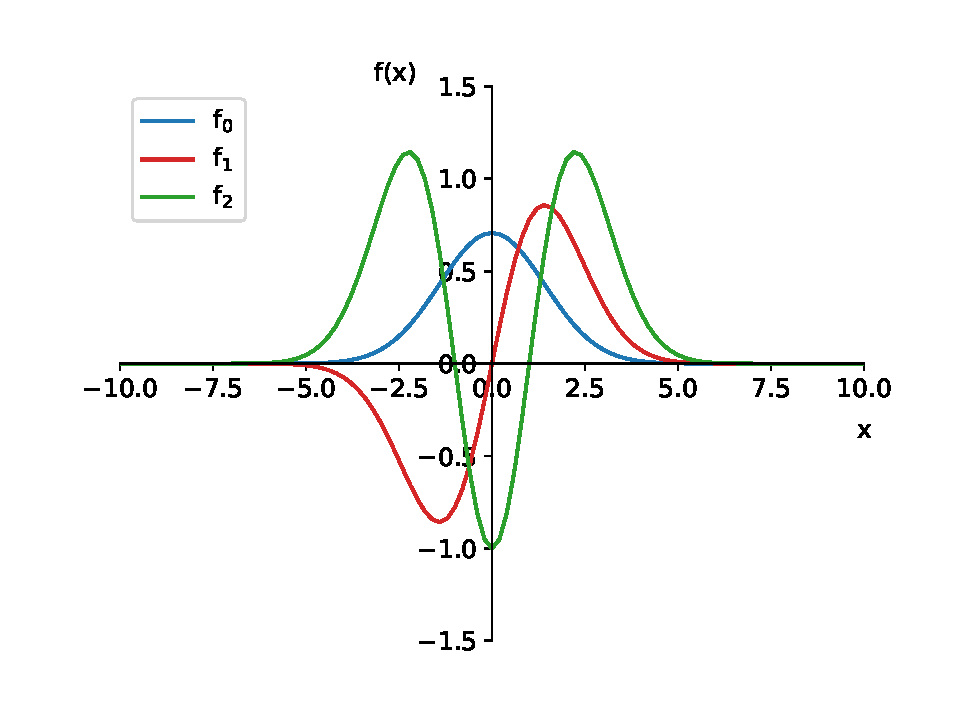
\includegraphics[width=\textwidth]{figures/appendices/herm_polys.pdf}
    \caption{Parabolic Cylinder Functions.}\label{fig:hermite-functions}
  \end{subfigure}
  \quad
  \begin{subfigure}[b]{0.48\textwidth}
    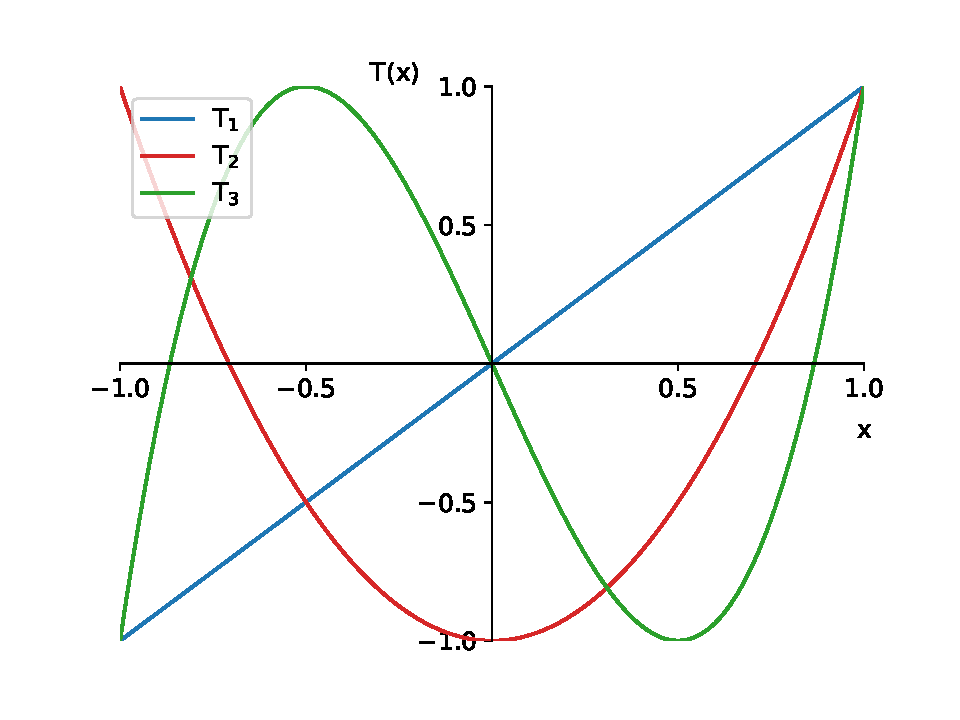
\includegraphics[width=\textwidth]{figures/appendices/cheb_polys.pdf}
    \caption{Chebyshev Polynomials.}\label{fig:chebyshev-polynomials}
  \end{subfigure}
\caption{The basis functions used for the pseudo-spectral methods to solve the shallow-water equations on a beta-plane and on a sphere. The choice of basis function depends primarily on the boundary conditions of the system.}\label{fig:basis-functions}
\end{figure}



\section{Spherical Shallow-Water Equations}
 %
 % \citet{boyd1978shearI} solves the linearized shallow-water equations, by reducing them to a single equation for a single variable, and applying the pseudo-spectral method. In this paper, we solve the entire system of shallow-water equations at once with the method in Appendix \ref{sec:app-systems}, but explain the method for a single equation here as it naturally leads to the second method \citep{boyd2000spectral}.
 %


 This method is used in Chapters \ref{ch:eqm-zonal-flow} and \ref{ch:wave-mean-flow} to solve the shallow-water equations on a sphere. These equations are singular with respect to $u$ and $v$ at the poles (although real solutions do exist), so all the variables cannot be solved simultaneously as on the beta-plane \citep{iga2005spherical}. Instead, the three shallow-water equations can be reduced to one equation in $\phi$, also known as ``Laplace's Tidal Equation'' \citep{pekeris1975laplace, dunkerton1990laplace}. This equation can be solved with a pseudo-spectral method, then the solution for $\phi$ used to find the solutions for $u$ and $v$.

 The linear shallow-water equations on the sphere are:

 \begin{equation}
   \begin{aligned}
     {\frac{\partial u^{\prime}}{\partial t}+\frac{\partial\left(\overline{U} u^{\prime}\right)}{a \cos \theta \partial \lambda}+v^{\prime} \frac{\partial \overline{U}}{a \partial \theta}-\frac{\overline{U} v^{\prime} \tan \theta}{a}=2 \Omega v^{\prime} \sin \theta-\frac{g \partial h^{\prime}}{a \cos \theta \partial \lambda}}, \\
      {\frac{\partial v^{\prime}}{\partial t}+\frac{\partial\left(\overline{U} v^{\prime}\right)}{a \cos \theta \partial \lambda}+\frac{2 \overline{U} u^{\prime} \tan \theta}{a}=-2 \Omega u^{\prime} \sin \theta-\frac{g \partial h^{\prime}}{a \partial \theta}}, \\
      {\frac{\partial h^{\prime}}{\partial t}+v^{\prime} \frac{\partial \overline{H}}{a \partial \theta}+\overline{U} \frac{\partial h^{\prime}}{a \cos \theta \partial \lambda}+\overline{H} \nabla_{H} \cdot \mathbf{v}^{\prime}=0},
   \end{aligned}
 \end{equation}

 where $h$ is the height of the layer, $\boldsymbol{v} = (u,v)$ is the velocity, $\theta$ is latitude, $\lambda$ is longitude, $t$ is time, $a$ is radius, $g$ is gravity, and $\Omega$ is angular velocity. Overbars denote zonal-mean quantities (the background flow and height $\overline{U}$ and $\overline{H}$). Dashes denote perturbations to this background state.

 The background state is stationary and the zonally uniform equatorial jet $\overline{U}$ is in gradient wind balance:

 \begin{equation}
   \frac{1}{a} \frac{\partial}{\partial \theta}\left(\overline{H}+h_{g}\right)=-\left(2 \Omega \overline{U} \sin \theta+\frac{\overline{U}^{2}}{a} \tan \theta\right).
 \end{equation}

 The perturbed variables are wavelike in longitude and are uniformly damped, so have the form $X(y) \exp [i m \lambda+\alpha t)]$. All variables are made non-dimensional with velocity scale $2 \Omega a$, height scale $(2 \Omega a)^{2}/g$ and time scale $1/(2\Omega)$, and denoted as such by an asterisk. This gives the following non-dimensional shallow-water equations:

 \begin{equation}
   \begin{aligned}
     \alpha^{*} u_{m}^{*}+i m \frac{\overline{U}^{*} u_{m}^{*}}{\cos \theta}+v_{m}^{*} \frac{\partial \overline{U}^{*}}{\partial \theta}-\overline{U}^{*} v_{m}^{*} \tan \theta &=v_{m}^{*} \sin \theta-\frac{i m h_{m}^{*}}{\cos \theta}, \\
     \alpha^{*} v_{m}^{*}+i m \frac{\overline{U}^{*} v_{m}^{*}}{\cos \theta}+2 \overline{U}^{*} u_{m}^{*} \tan \theta &=-u_{m}^{*} \sin \theta-\frac{\partial h_{m}^{*}}{\partial \theta}, \\
     \alpha^{*} h_{m}^{*}+i m \overline{U}^{*} \frac{h_{m}^{*}}{\cos \theta} &=-\frac{\epsilon^{*}}{\cos \theta}\left[i m u_{m}^{*}+\frac{\partial}{\partial \theta}\left(\cos \theta v_{m}^{*}\right)\right],
   \end{aligned}
 \end{equation}

 where Lamb's parameter is $\epsilon \equiv(2 \Omega a)^{2} / g H$. These can be written as

 \begin{equation}
   \begin{aligned}
     - \hat{\sigma}^{*} u_{m}^{*} - \overline{\zeta}^{*}v_{m}^{*} + \frac{m h_{m}^{*} }{\cos \theta} = 0, \\
     \hat{\sigma}^{*}  v_{m}^{*} + f_{1}^{*}u_{m}^{*} + \frac{d h_{m}^{*}}{d \theta} = 0, \\
     \hat{\sigma}^{*}  \epsilon \alpha h_{m}^{*}+ \frac{m u_{m}^{*}}{\cos \theta} + \frac{1}{\cos \theta} \frac{d}{d \theta}(v \cos \theta) = 0,
   \end{aligned}
 \end{equation}

 where

 \begin{equation}
     \overline{\zeta}^{*} = f^{*} - \frac{1}{\cos \theta} \frac{d}{d \theta}(\overline{U} \cos \theta)
 \end{equation}

 is the absolute vorticity of the background flow,

 \begin{equation}
     f_{1} = f + 2 \overline{U} \tan \theta
 \end{equation}

 is an effective Coriolis parameter modified by the background flow, and

 \begin{equation}
     \hat{\sigma}^{*}  =  \sigma^{*} - \frac{m \overline{U}}{\cos \theta}
 \end{equation}

 is the Doppler-shifted time-derivative of the variables (see Chapter \ref{ch:wave-mean-flow}). Solving the first two shallow-water equations gives the two velocity components in terms of the height field:

 \begin{equation}
   \begin{aligned}
     u_{m}^{*} = \frac{- \hat{\sigma}^{*}h_{m}^{*} m/\cos \theta - \overline{\zeta}^{*} d h_{m}^{*} / d y}{\Delta},\\
     v_{m}^{*} = \frac{\hat{\sigma}^{*} d h_{m}^{*} / d y + f_{1}^{*} h_{m}^{*} m / \cos \theta }{\Delta}.
   \end{aligned}
 \end{equation}

 where $\Delta = f_{1}^{*} \overline{\zeta}^{*} - \hat{\sigma}^{*2}$. Then, substituting these into the third shallow-water equation, while changing variables to $\mu = \sin \theta$ and $\phi_{m}^{*} = \left(1-\mu^{2}\right)^{-m / 2} h_{m}^{*}$ to avoid the polar singularities \citep{iga2005spherical}, gives:


 \begin{equation}
   \frac{\partial^{2} \phi_{m}^{*}}{\partial \mu^{2}}-B\left(\sigma^{*}, \mu\right) \frac{\partial \phi_{m}^{*}}{\partial \mu}-A\left(\sigma^{*}, \mu\right) \phi_{m}^{*}=\frac{F(\theta,x)}{i \sigma},
 \end{equation}

 where

 \begin{equation}
   \begin{aligned} A\left(\sigma^{*}, \mu\right) \equiv & \frac{1}{1-\mu^{2}}\left[m(m+1)-m \mu \frac{1}{\Delta^{*}} \frac{\partial \Delta^{*}}{\partial \mu}+\epsilon \Delta^{*}\right.\\ &+\frac{m}{\Delta^{*} \hat{\sigma}^{*}}\left(f_{1}^{*} \frac{\partial \Delta^{*}}{\partial \mu}-\Delta * \frac{\partial f_{1}^{*}}{\partial \mu}\right) ], \\ B\left(\sigma^{*}, \mu\right) & \equiv \frac{1}{\Delta^{*}} \frac{\partial \Delta^{*}}{\partial \mu}+\frac{2 \mu(m+1)}{\left(1-\mu^{2}\right)}, \\ \Delta^{*} & \equiv f_{1}^{*} \overline{\zeta}^{*}-\hat{\sigma}^{* 2}. \end{aligned}
 \end{equation}

 This equation is then solved with a pseudo-spectral method using the Chebyshev polynomials plotted in Figure \ref{fig:basis-functions} \citep{wang2016hough}. The tidal equation in spherical coordinates can be modified to represent the beta-plane by setting $\cos \theta = 1$ and $f_{1} = f$ \citep{dunkerton1990laplace}.


%
% \section{Solving the Shallow-Water Equations}
%
% This method is used in Chapter X.
%
% We use the \textbf{parabolic cylinder functions} $\psi_{n}(y)$ \citep{showman2011superrotation} as defined in Equation \ref{eqn:hermite-functions} as a basis set for the pseudo-spectral method on the beta-plane (Equation \ref{eqn:forced-sw}), as they are the exact free solutions of \citet{matsuno1966quasi} \citep{boyd2000spectral}.
%
% Their collocation points are at their zeros (which are just the zeros of the Hermite polynomials $H_{n}$). Figure \ref{fig:hermite-functions} shows the first few \textbf{parabolic cylinder functions}.
%
% \begin{equation}\label{eqn:hermite-functions}
%   \psi_{n}(y) = e^{-y^{2} / 2} H_{n}(y)
% \end{equation}
%
% Figure \ref{fig:accuracy-hermite} shows the magnitude of the coefficients (Equation \ref{eqn:ps-coeff-solutions}) of the pseudo-spectral solution of the shallow-water equations linearized about a jet on a beta-plane (plotted in Figure \ref{fig:shear-2D}). The first plot shows that when the background jet flow is zero, only modes up to $n=2$ are non-zero. This is the analytic solution from \citet{matsuno1966quasi}, which the pseudo-spectral method identifies because we have used the free modes (the \textbf{parabolic cylinder functions}) as our basis functions.
%
% For non-zero jet speed (corresponding to Figure \ref{fig:shear-2D}), the pseudo-spectral series solution does not terminate, but the coefficients for the 30th mode are about eight orders of magnitude smaller than the largest mode. The beta-plane solutions in this paper were all calculated with at least 30 modes.
%
% This method is not as effective in a spherical geometry due to singularities in the equations at the poles. In the next section, I will show how the three shallow-water equations can be reduced to a single tidal equation that avoids these singularities, then solved in the same way.
%
% \begin{figure}
%     \centering
%   \begin{subfigure}[b]{0.4\textwidth}
%     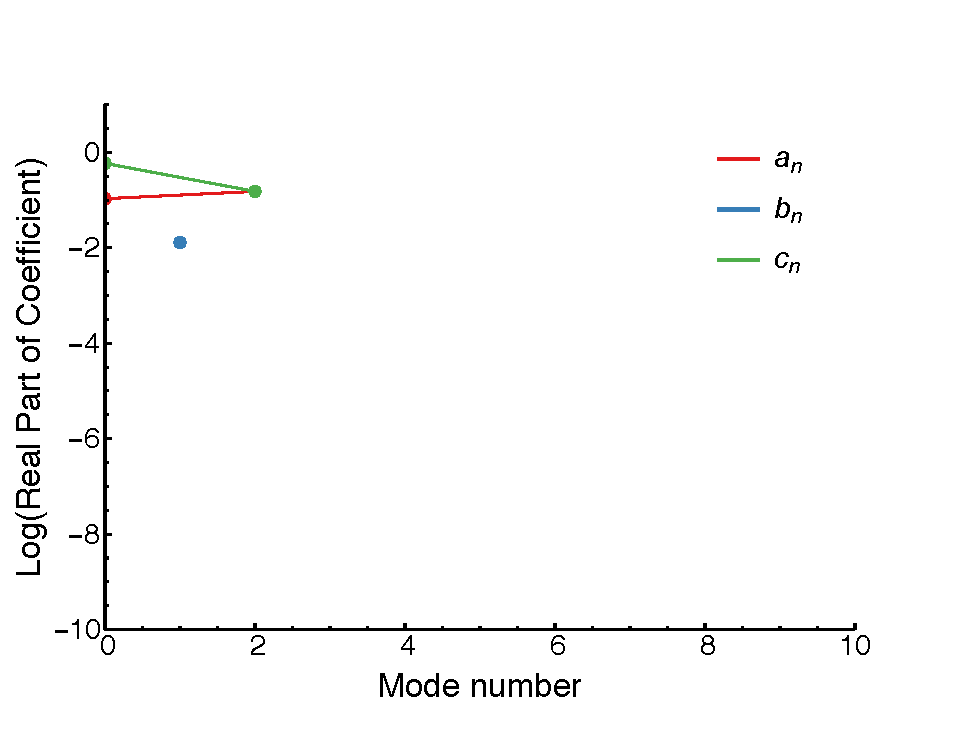
\includegraphics[width=\textwidth]{figures/appendices/zero-shear-hermite-accuracy.pdf}
%     \caption{Coefficients for $\bar{U}(y)=0$.}
%   \end{subfigure}
%   %
%   \begin{subfigure}[b]{0.4\textwidth}
%     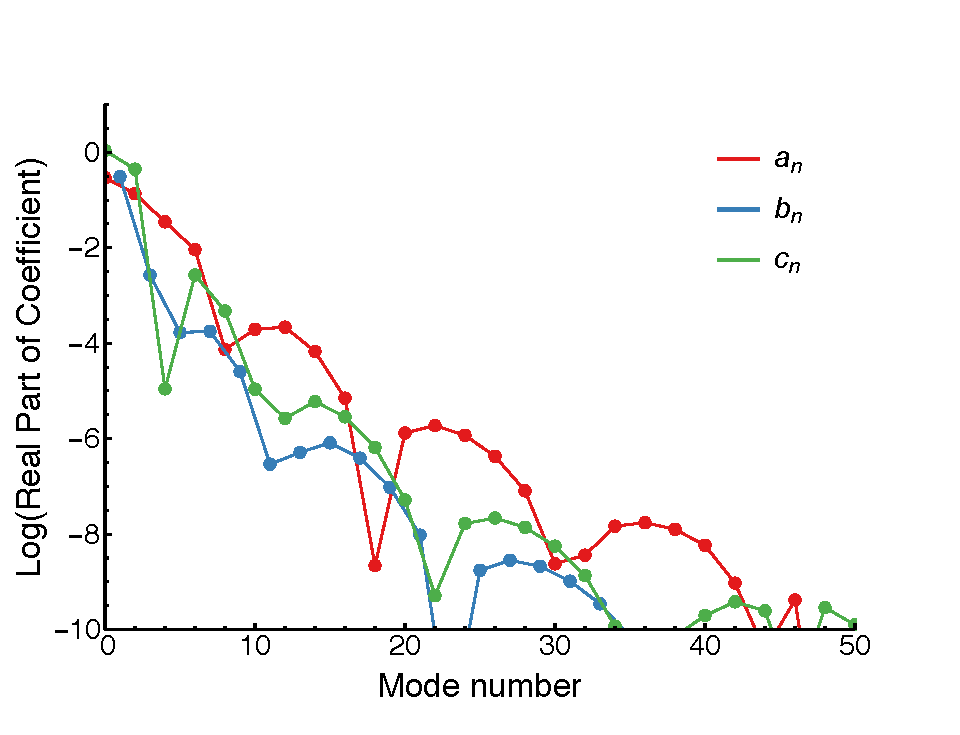
\includegraphics[width=\textwidth]{figures/appendices/shear-hermite-accuracy.pdf}
%     \caption{Coefficients for $\bar{U}(y)=\exp(-y^{2}/2)$.}
%   \end{subfigure}
% \caption{Coefficients of the pseudo-spectral solution on the beta-plane coordinates with and without a background jet (the plots in Figure \ref{fig:shear-2D}). The method identifies the exact solution in the first case, and converges rapidly to an accurate solution in the second case. }\label{fig:accuracy-hermite}
% \end{figure}

% \section{Solving a Single Tidal Equation}\label{ap:tidal-eqn}
%
%
% \subsection*{Collocation}
%
% \citep{wang2016hough}
%
% \subsection*{Solutions}
%
% The full solutions are reconstructed
%
% \subsection*{Special Cases}
%
% \subsubsection{Equatorial Beta-Plane}
%




%
% \section{Example Solutions}
%
%
% \subsection*{Beta-plane solutions}\label{sec:app-beta}
%
% We use the \textbf{parabolic cylinder functions} $\psi_{n}(y)$ \citep{showman2011superrotation} as defined in Equation \ref{eqn:hermite-functions} as a basis set for the pseudo-spectral method on the beta-plane (Equation \ref{eqn:forced-sw}), as they are the exact free solutions of \citet{matsuno1966quasi} \citep{boyd2000spectral}.
%
% Their collocation points are at their zeros (which are just the zeros of the Hermite polynomials $H_{n}$). Figure \ref{fig:hermite-functions} shows the first few \textbf{parabolic cylinder functions}.
%
% \begin{equation}\label{eqn:hermite-functions}
%   \psi_{n}(y) = e^{-y^{2} / 2} H_{n}(y)
% \end{equation}
%
% Figure \ref{fig:accuracy-hermite} shows the magnitude of the coefficients (Equation \ref{eqn:ps-coeff-solutions}) of the pseudo-spectral solution of the shallow-water equations linearized about a jet on a beta-plane (plotted in Figure \ref{fig:shear-2D}). The first plot shows that when the background jet flow is zero, only modes up to $n=2$ are non-zero. This is the analytic solution from \citet{matsuno1966quasi}, which the pseudo-spectral method identifies because we have used the free modes (the \textbf{parabolic cylinder functions}) as our basis functions.
%
% For non-zero jet speed (corresponding to Figure \ref{fig:shear-2D}), the pseudo-spectral series solution does not terminate, but the coefficients for the 30th mode are about eight orders of magnitude smaller than the largest mode. The beta-plane solutions in this paper were all calculated with at least 30 modes.
%
% \begin{figure}
%     \centering
%   \begin{subfigure}[b]{0.4\textwidth}
%     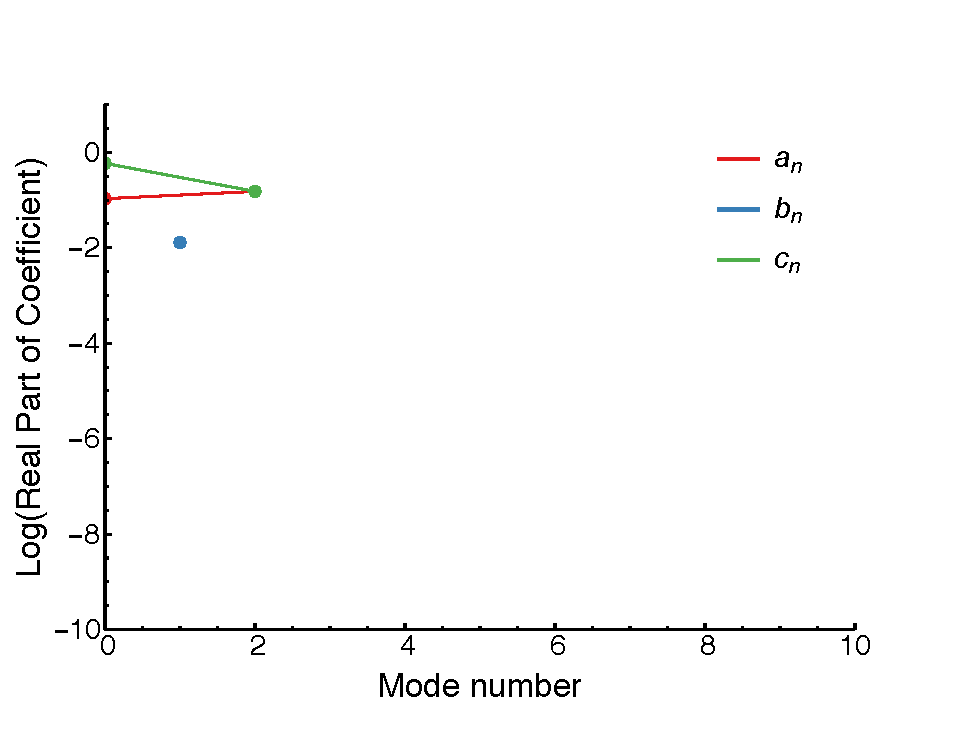
\includegraphics[width=\textwidth]{figures/appendices/zero-shear-hermite-accuracy.pdf}
%     \caption{Coefficients for $\bar{U}(y)=0$.}
%   \end{subfigure}
%   %
%   \begin{subfigure}[b]{0.4\textwidth}
%     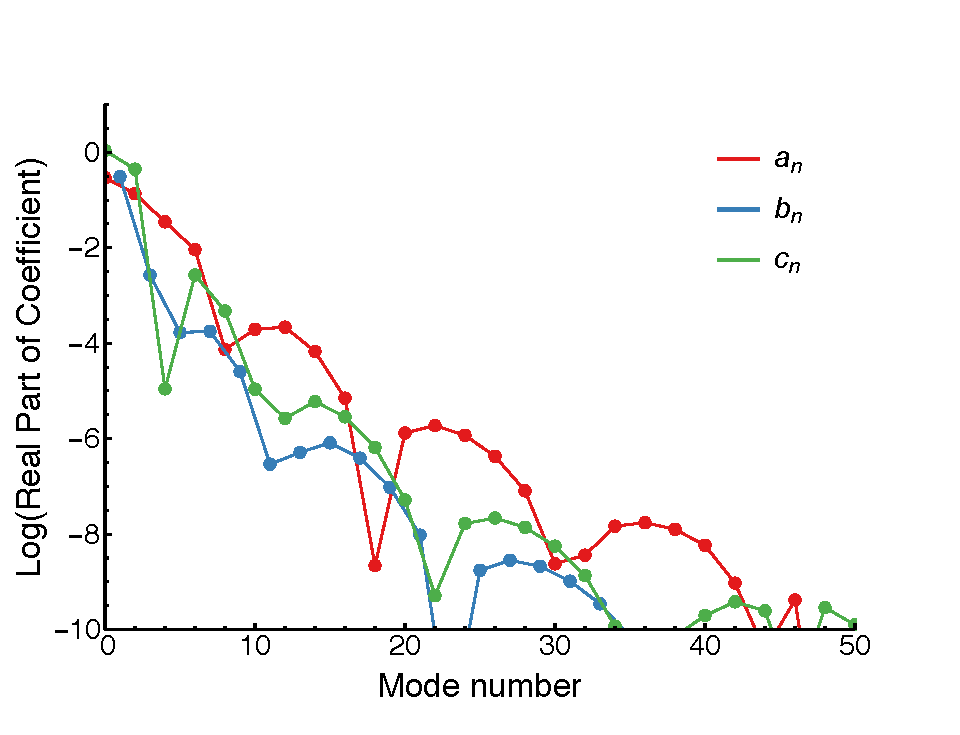
\includegraphics[width=\textwidth]{figures/appendices/shear-hermite-accuracy.pdf}
%     \caption{Coefficients for $\bar{U}(y)=\exp(-y^{2}/2)$.}
%   \end{subfigure}
% \caption{Coefficients of the pseudo-spectral solution on the beta-plane coordinates with and without a background jet (the plots in Figure \ref{fig:shear-2D}). The method identifies the exact solution in the first case, and converges rapidly to an accurate solution in the second case. }\label{fig:accuracy-hermite}
% \end{figure}
%
%
% \subsection*{Spherical solutions}\label{sec:app-spherical}
%
% We use the Legendre polynomials as a basis set for the pseudo-spectral method in a spherical geometry (Equation \ref{eqn:sphere-sw-eqns}). Figure \ref{fig:legendre-polynomials} shows the first few Legendre polynomials. Our collocation points are the zeros of these functions.
%
% As discussed in Section \ref{sec:sphere-solutions}, Equation \ref{eqn:sphere-sw-eqns} has a singularity at the poles, which we avoided by using a rescaled height $\gamma$, where $\gamma = h / \cos\phi$ \citep{iga2005spherical}. We replaced $h$ with $\gamma \cos \phi$ in Equation \ref{eqn:sphere-sw-eqns}, solved as normal, then multiplied the solution for $\gamma$ by $\cos\phi$ to recover the solution for $h$.
%
% Figure \ref{fig:accuracy-spherical} shows how rescaling the $h$ variable made the solutions converge much more quickly. In fact, the solutions without a rescaled $h$ variable never reached a smooth solution at the poles.
%
%
% \begin{figure}
%     \centering
%   \begin{subfigure}[b]{0.4\textwidth}
%     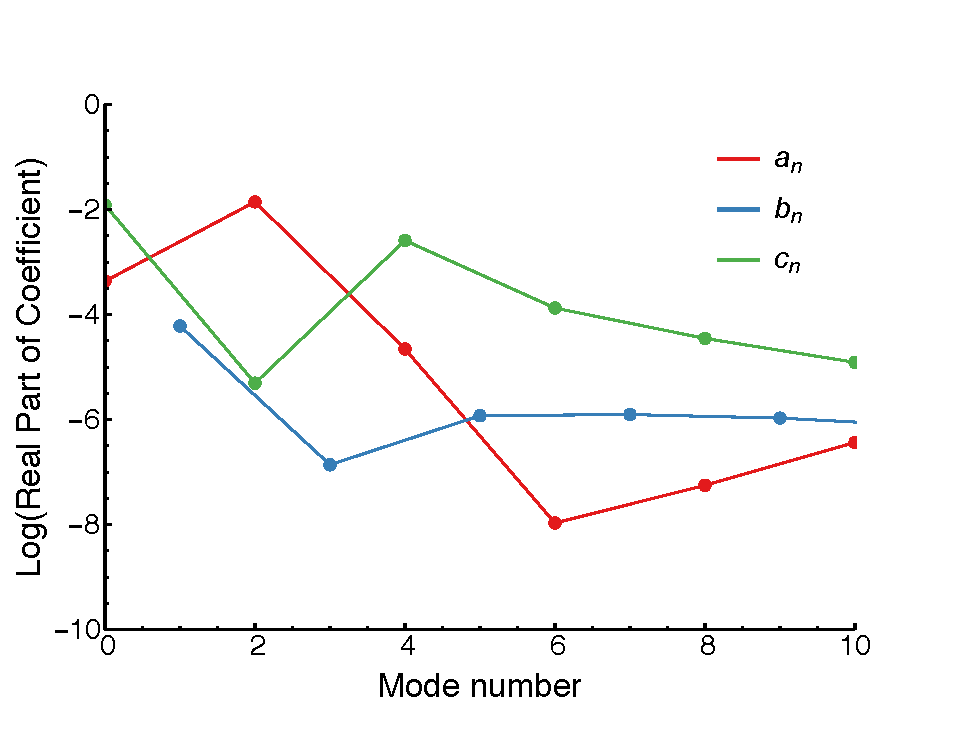
\includegraphics[width=\textwidth]{figures/appendices/sphere-accuracy-noscale.pdf}
%     \caption{Coefficients calculated with height $h$.}
%   \end{subfigure}
%   %
%   \begin{subfigure}[b]{0.4\textwidth}
%     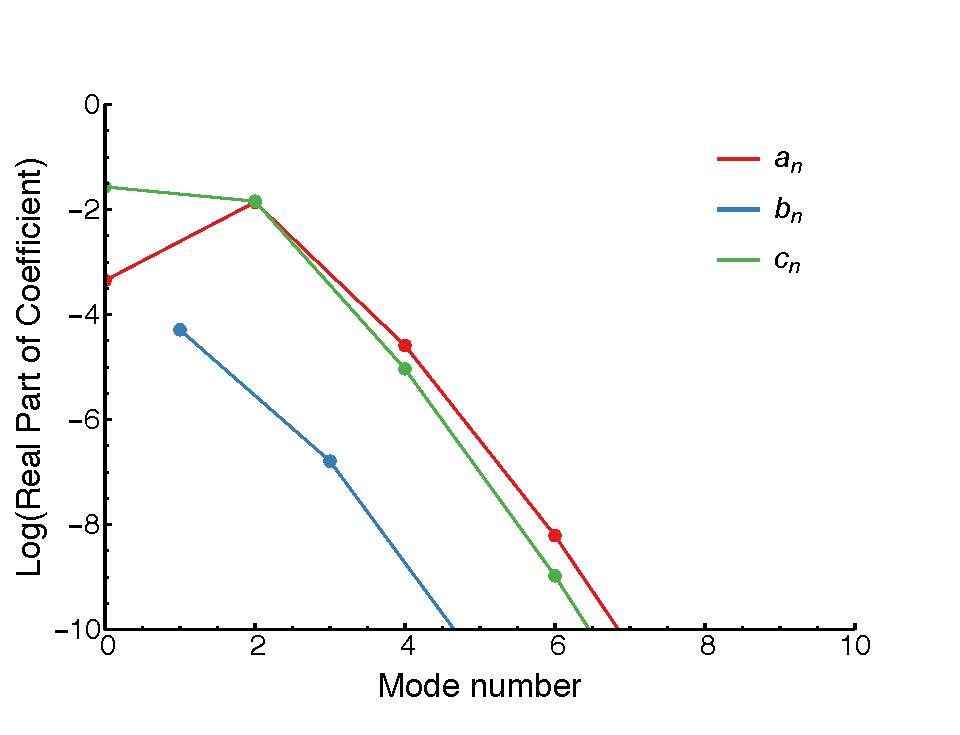
\includegraphics[width=\textwidth]{figures/appendices/sphere-accuracy-rescale.pdf}
%     \caption{Coefficients calculated with rescaled height $\gamma = h / \cos\phi$.}
%   \end{subfigure}
% \caption{Coefficients of the pseudo-spectral solution in spherical coordinates (the first plot in Figure \ref{fig:spherical-tests}), with the height variable $h$ and the rescaled height $\gamma$. Rescaling the height makes the method converge to a smooth solution at the poles.}\label{fig:accuracy-spherical}
% \end{figure}


% \bibliographystyle{unsrtnat}
% \bibliography{references.bib}
